%!TEX root = ../../main.tex
\section{RSConverter}
RS485-bussen er valgt til at kommunikere på, se hvorfor i teknologiundersøgelsen. Til dette formål er udformet et simpelt kredsløb vha. MAX3082. Det logiske 0-5V UART-signal fra PSoC 4 konverteres til et differentielt signal, som kører ud på bussen, og vice versa.

\begin{figure}[H]
	\centering
	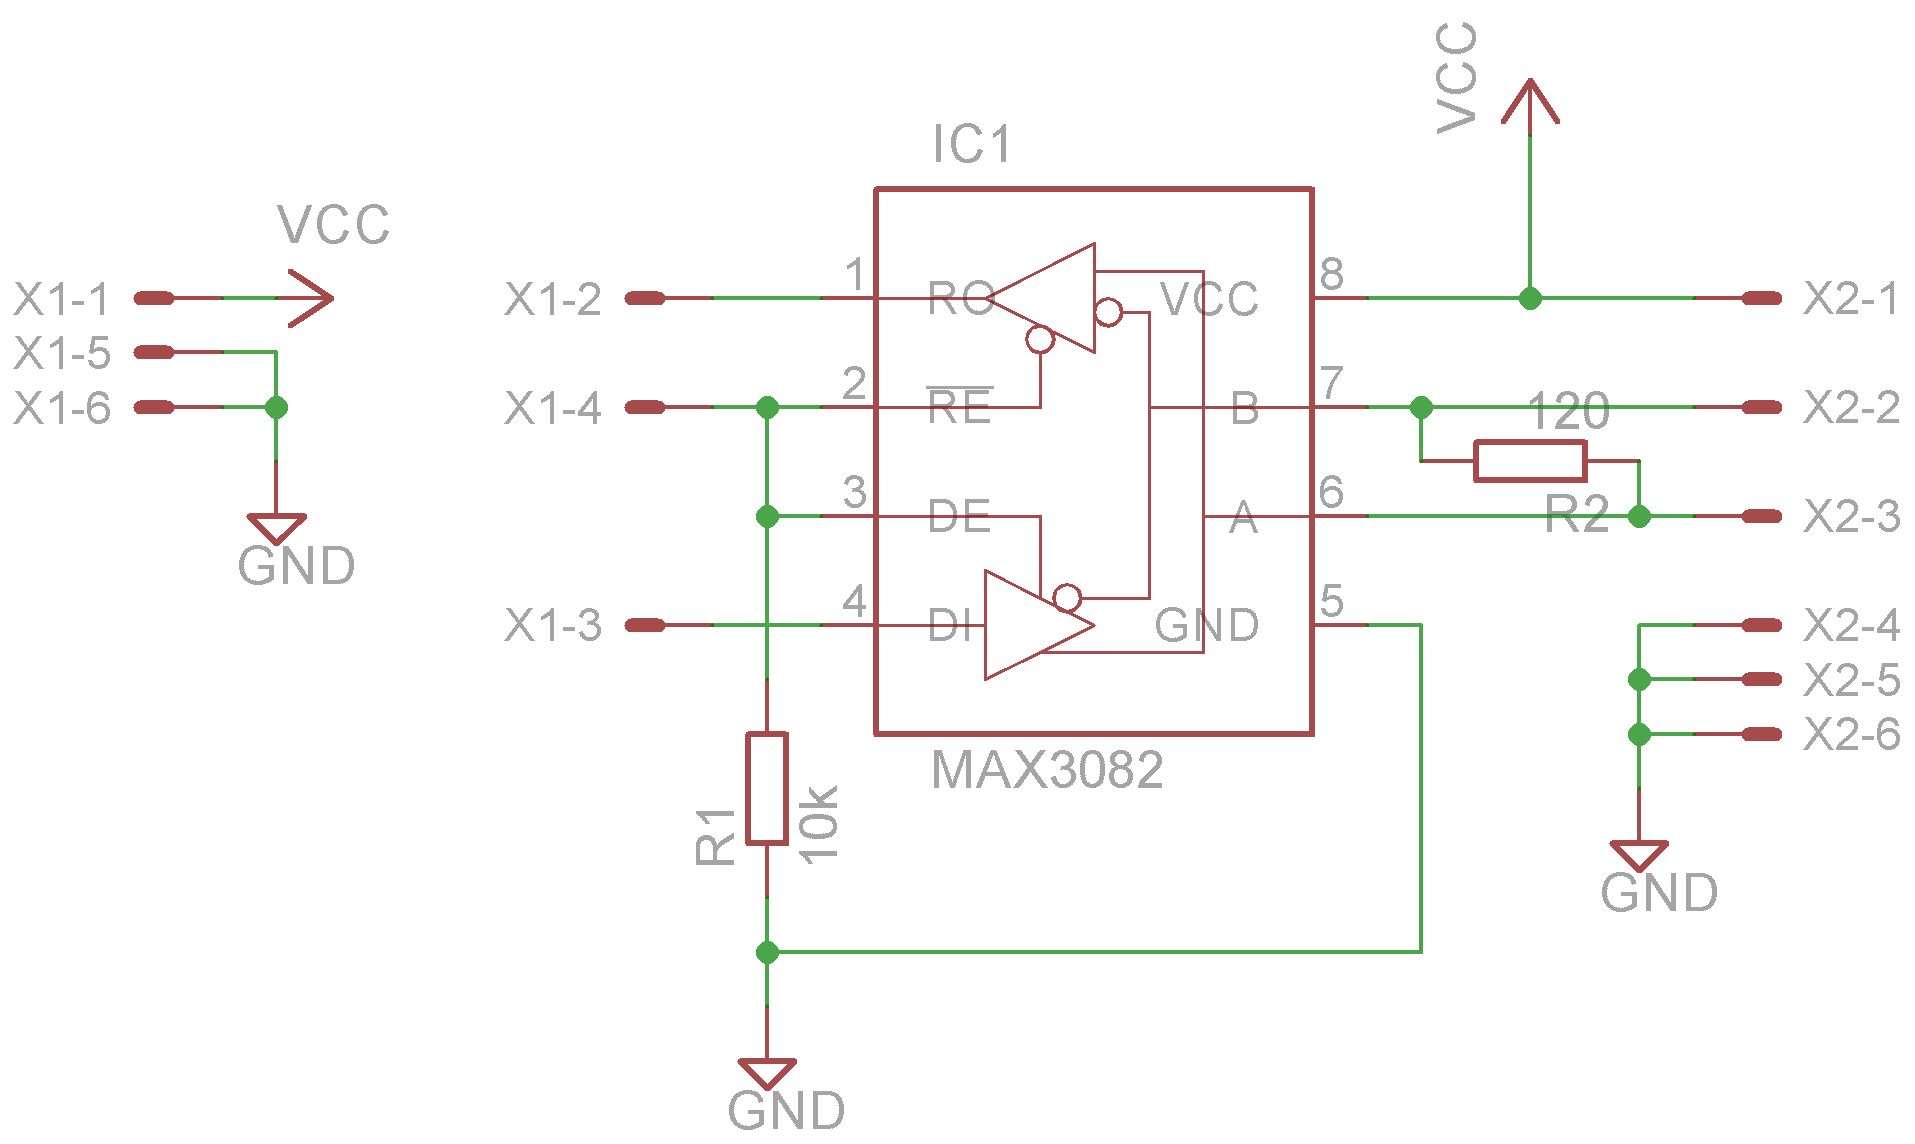
\includegraphics[scale=1]{../Hardware/RS485_Converter/Schematic}
	\caption{RS485 converter}
	\label{photo:RS485converter}
\end{figure}

For at udregne det maksimale strømforbrug kigges i databladet for MAX3082. Under "Absolute Maximum Ratings" findes det, at i et 8-pin plastic DIP hus som det der anvendes, har et typisk effekt forbrug på 727mW.

Udregningen af det maksimale strømforbrug bliver derfor følgende:
\begin{equation}
	I = \frac{P}{U} = \frac{727mW}{5V} = 145,4mA
\end{equation}

\fxnote{Scopebilleder, forklaringer osv.}